\newcommand{\computationalPIR}{
    \begin{figure}
        \centering
        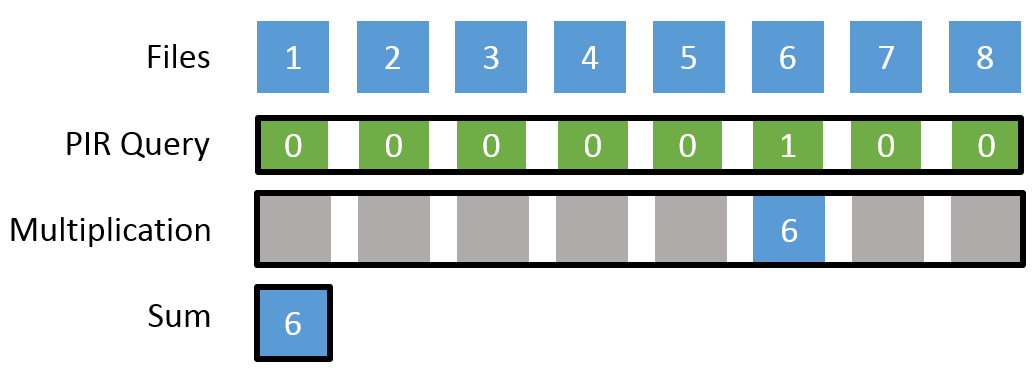
\includegraphics[width=\linewidth]{figs/pir-basic}
        \caption{Computational PIR leverages homomorphic encryption to make private queries to a database. A user encrypts a vector of 0s and a 1 corresponding to the desired entry, the server can then leverage homomorphic multiplication and homomorphic addition to return the requested entry without learning what was requested.}
        \label{fig:cpir}
    \end{figure}
}

\newcommand{\DCNet}{
    \begin{figure}
        \centering
        \begin{subfigure}{0.5\textwidth}
            \centering
            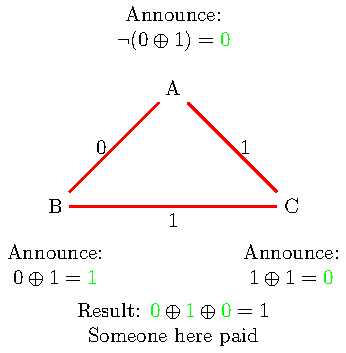
\includegraphics[width=0.6\linewidth]{figs/DCTriangleApaid}
            \caption{A simple Boolean DC-Net}
            \label{fig:simpleDCNet}
        \end{subfigure}%
        \begin{subfigure}{0.5\textwidth}
            \centering
            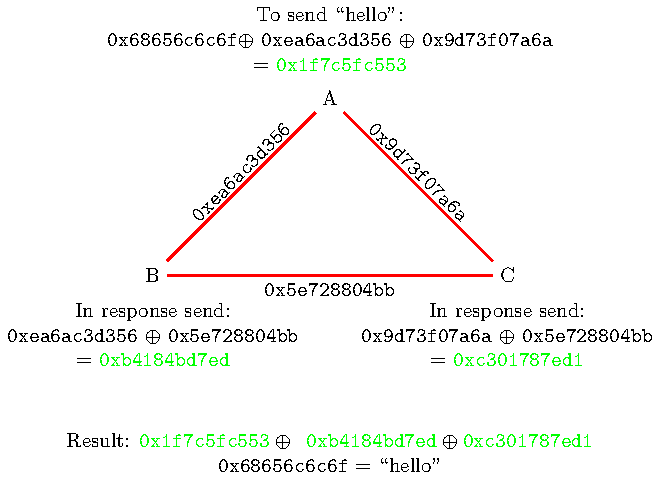
\includegraphics[width=0.85\linewidth]{figs/DCTriangleMessage}
            \caption{A more complicated message DC-Net}
            \label{fig:messageDCNet}
        \end{subfigure}% 
        \caption{Dining Cryptographer networks allow anonymous
        communication by having shared secrets between all users. In (a) three
        users at a dinner that has been anonymously paid for can determine
        whether someone at the table or the NSA paid for the meal while
        maintaining the payers anonymity. Each user flips a coin to get a shared
        bit with each other user and then \texttt{xor}s the shared secrets they
        know and announces the result. The user attempting to announce they have
        paid (anonymously) for a meal can flip their response. All announced
        bits are \texttt{xor}ed and a result of 1 means someone at the table
        paid, though no one knows who. In (b) this generalizes to allow
        anonymous communication. Each user generates a shared bitstream with
        every other participant and announces the \texttt{xor} of all shared
        secrets. The user sending a message first \texttt{xor}s in their message
        as well and announces. All announced messages are \texttt{xor}ed and the result is the sent message.}
        \label{fig:dcnet}
    \end{figure}
}